% This is the Reed College LaTeX thesis template. Most of the work
% for the document class was done by Sam Noble (SN), as well as this
% template. Later comments etc. by Ben Salzberg (BTS). Additional
% restructuring and APA support by Jess Youngberg (JY).
% Your comments and suggestions are more than welcome; please email
% them to cus@reed.edu
%
% See https://www.reed.edu/cis/help/LaTeX/index.html for help. There are a
% great bunch of help pages there, with notes on
% getting started, bibtex, etc. Go there and read it if you're not
% already familiar with LaTeX.
%
% Any line that starts with a percent symbol is a comment.
% They won't show up in the document, and are useful for notes
% to yourself and explaining commands.
% Commenting also removes a line from the document;
% very handy for troubleshooting problems. -BTS

% As far as I know, this follows the requirements laid out in
% the 2002-2003 Senior Handbook. Ask a librarian to check the
% document before binding. -SN

%%
%% Preamble
%%
% \documentclass{<something>} must begin each LaTeX document
\documentclass[12pt,twoside]{templates/facsothesis}
% Packages are extensions to the basic LaTeX functions. Whatever you
% want to typeset, there is probably a package out there for it.
% Chemistry (chemtex), screenplays, you name it.
% Check out CTAN to see: https://www.ctan.org/
%%
\ifxetex
  \usepackage{polyglossia}
  \setmainlanguage{spanish}
  % Tabla en lugar de cuadro
  \gappto\captionsspanish{\renewcommand{\tablename}{Tabla}
          \renewcommand{\listtablename}{Índice de tablas}}
\else
  \usepackage[spanish,es-tabla]{babel}
\fi
%\usepackage[spanish]{babel}
\usepackage{graphicx,latexsym}
\usepackage{amsmath}
\usepackage{amssymb,amsthm}
\usepackage{longtable,booktabs,setspace}
\usepackage{chemarr} %% Useful for one reaction arrow, useless if you're not a chem major
\usepackage[hyphens]{url}
% Added by CII
%\usepackage{hyperref}
\usepackage[colorlinks = true,
            linkcolor = blue,
            urlcolor  = blue,
            citecolor = blue,
            anchorcolor = blue]{hyperref}
\usepackage{lmodern}
\usepackage{float}
\floatplacement{figure}{H}
% End of CII addition
\usepackage{rotating}
\usepackage{placeins} % para fijar la posición de las tablas con \FloatBarrier


\usepackage[]{natbib}


% Next line commented out by CII
%\usepackage{biblatex}
%\usepackage{natbib}
% Comment out the natbib line above and uncomment the following two lines to use the new
% biblatex-chicago style, for Chicago A. Also make some changes at the end where the
% bibliography is included.
%\usepackage{biblatex-chicago}
%\bibliography{thesis}


% Added by CII (Thanks, Hadley!)
% Use ref for internal links
\renewcommand{\hyperref}[2][???]{\autoref{#1}}
\def\chapterautorefname{Chapter}
\def\sectionautorefname{Section}
\def\subsectionautorefname{Subsection}
% End of CII addition

% Added by CII
\usepackage{caption}
\captionsetup{width=5in}
% End of CII addition

% \usepackage{times} % other fonts are available like times, bookman, charter, palatino

% Syntax highlighting #22

% To pass between YAML and LaTeX the dollar signs are added by CII
\title{Aceptar la diversidad en el vecindario}
\author{Kevin Carrasco Quintanilla}
% The month and year that you submit your FINAL draft TO THE LIBRARY (May or December)
\date{2022-05-29}
\division{}
\advisor{Profesor guía: Juan Carlos Castillo}
\institution{Universidad de Chile}
\degree{Magister en ciencias sociales mención en sociología de la modernización}
%If you have two advisors for some reason, you can use the following
% Uncommented out by CII
% End of CII addition

%%% Remember to use the correct department!
\department{}
% if you're writing a thesis in an interdisciplinary major,
% uncomment the line below and change the text as appropriate.
% check the Senior Handbook if unsure.
%\thedivisionof{The Established Interdisciplinary Committee for}
% if you want the approval page to say "Approved for the Committee",
% uncomment the next line
%\approvedforthe{Committee}

% Added by CII
%%% Copied from knitr
%% maxwidth is the original width if it's less than linewidth
%% otherwise use linewidth (to make sure the graphics do not exceed the margin)
\makeatletter
\def\maxwidth{ %
  \ifdim\Gin@nat@width>\linewidth
    \linewidth
  \else
    \Gin@nat@width
  \fi
}
\makeatother

%Added by @MyKo101, code provided by @GerbrichFerdinands

\setlength\parindent{0pt}


% Added by CII

\providecommand{\tightlist}{%
  \setlength{\itemsep}{0pt}\setlength{\parskip}{0pt}}

\Acknowledgements{

}

\Dedication{

}

\Preface{

}

\Abstract{

}

	\usepackage{booktabs}
 \usepackage{longtable}
 \usepackage{array}
 \usepackage{multirow}
 \usepackage{wrapfig}
 \usepackage{float}
 \usepackage{colortbl}
 \usepackage{pdflscape}
 \usepackage{tabu}
 \usepackage{threeparttable}
 \usepackage{threeparttablex}
 \usepackage[normalem]{ulem}
 \usepackage{makecell}
 \usepackage{xcolor}
% End of CII addition
%%
%% End Preamble
%%
%
\let\chaptername\relax
\begin{document}
\bibliographystyle{apalike}
% Everything below added by CII
  \maketitle

\frontmatter % this stuff will be roman-numbered
\pagestyle{empty} % this removes page numbers from the frontmatter



%  \hypersetup{linkcolor=black}
  \setcounter{tocdepth}{1}
  \setlength{\parskip}{0pt}
  \tableofcontents

\setlength\parskip{1em plus 0.1em minus 0.2em}

  \listoftables

  \listoffigures



\mainmatter % here the regular arabic numbering starts
\pagestyle{fancyplain} % turns page numbering back on

\hypertarget{resumen}{%
\chapter{Resumen}\label{resumen}}

Abordar el aprendizaje de actitudes hacia la diversidad social de jóvenes en edad escolar implica posicionar esta investigación bajo un incremento de la diversidad social que plantea importantes desafíos para los Estados-nación a nivel global en términos de políticas públicas, ya sea por sus implicancias gubernamentales, territoriales y socioeconómicas, como también por los nuevos requisitos que se originan en los distintos sistemas educativos a partir de demandas por inclusión y tolerancia de una población estudiantil diversa. Hasta ahora, las investigaciones sobre diversidad social se han situado frecuentemente bajo el paradigma de la integración social, es decir, en la forma en que distintos grupos sociales poseen determinada posición dentro de la estructura social (ej. Young 2000; Wade 2000; Viveros Vigoya 2016). Al situarse bajo este paradigma, se han dejado de lado dos elementos fundamentales. Por un lado, se ha estudiado en menor medida el proceso de inclusión social en las escuelas (Blanco, 2006) y la percepción que la población tiene sobre los demás grupos, en el sentido de si aceptan o rechazan a determinados grupos sociales que son distintos o que poseen otras posiciones en la estructura social. Por otro lado, tampoco se ha abordado completamente el proceso mediante el cual se aprenden o reproducen en la sociedad las actitudes de las personas en relación con estos grupos sociales. Para la sociología la comprensión de la educación como un agente de socialización de las generaciones más jóvenes resulta fundamental, donde específicamente los aprendizajes que se le adjudican a la educación ciudadana en las escuelas buscan dar respuesta a la necesidad de preparar a la nueva generación para la vida en democracia y sus requerimientos morales y cognitivos (Cox y García 2015). Asimismo, dentro de la sociología el rol de la familia ha sido estudiado en menor medida, donde algunas investigaciones han dado cuenta del efecto de las actitudes de los padres en el conflicto interétnico de su descendencia (Medjedovic and Petrovic 2021) y de la participación política parental en el compromiso político de las nuevas generaciones (Bacovsky and Fitzgerald 2021). De esta forma, esta investigación pretende abordar estas dos problemáticas en su conjunto, es decir, se pretende abordar si jóvenes en edad escolar aceptan o rechazan a diferentes grupos sociales y los distintos procesos de socialización que están implicados en el aprendizaje de estas actitudes. Específicamente, mediante metodologías cuantitativas se espera demostrar que la familia y la escuela influyen en el proceso de aprendizaje de actitudes, donde además se espera que la escuela logre disminuir las desigualdades de origen. Los datos por utilizar provienen del primer estudio de Formación Ciudadana de Chile en 2017. Se cuenta con las respuestas de 8701 estudiantes y 6770 apoderados, provenientes de 242 escuelas del país.

\hypertarget{introducciuxf3n}{%
\chapter{Introducción:}\label{introducciuxf3n}}

Los procesos de modernización y globalización en Chile y Latinoamérica han planteado distintos desafíos tanto para lograr sus objetivos como por los resultados adversos que de ellos provienen. Según \citet{sunkel_sostenibilidad_1998}, el Siglo XXI comienza bajo una lógica de Apartheid, donde se crea un fenómeno de polarización en el que, por un lado, se genera un mejoramiento de la vida de segmentos muy limitados de la sociedad al tener una economía que crea muy poco empleo y, por otro lado, se genera exclusión social en segmentos crecientes de la población. Esta lógica dual también es retomada por \citet{castells_globalizacion_2005} al plantear que como la globalización es un instrumento de articulación de mercados capitalistas, la rentabilidad económica se convierte en el criterio fundamental para la inclusión o exclusión en las redes globales (donde se articulan o excluyen a ciertos individuos, grupos, países, regiones, etc.). En resumen, es el mismo proceso de globalización el que provoca y/o agrava los procesos de descomposición social \citep{lechner_debate_1992}.

Hasta ahora, las investigaciones sobre exclusión social se han situado frecuentemente bajo el paradigma de la integración social, es decir, en la forma en que distintos grupos sociales poseen determinada posición dentro de la estructura social \citep[ej.][]{young_justicia_2000, wade_raza_2000, viverosvigoya_interseccionalidad_2016}. Al situarse bajo este paradigma, se han dejado de lado dos elementos fundamentales. Por un lado, se ha estudiado en menor medida el proceso de inclusión social en las escuelas \citep{blanco_equidad_2006} y la percepción que la población tiene sobre los demás grupos, en el sentido de si aceptan o rechazan a determinados grupos sociales que son distintos o que poseen otras posiciones en la estructura social. Por otro lado, tampoco se ha abordado completamente el proceso mediante el cual se aprenden o reproducen en la sociedad las actitudes de las personas en relación con la aceptación o rechazo de determinados grupos sociales. De esta forma, esta investigación pretende abordar estas dos problemáticas en su conjunto, es decir, se pretende abordar si jóvenes en edad escolar aceptan o rechazan a diferentes grupos sociales y los distintos procesos de socialización que están implicados en el aprendizaje de estas actitudes.

Siguiendo el panorama mundial, con el aumento sostenido del desarrollo económico de los últimos años, se ha pasado de demandas sociales que apuntan a valores de supervivencia (demandas socioeconómicas, derechos sociales, acceso a servicios básicos, etc.) hacia demandas de auto expresión, creatividad y democratización que ayudan a remodelar las normas sexuales, los roles de género, los valores familiares, la religiosidad, la relación de las personas con la naturaleza y sus actividades comunitarias \citep{inglehart_Modernization_2001}, como tal, se han planteado importantes desafíos en términos de Democracia y Ciudadanía. Así, en cuanto a la aceptación o rechazo de determinados grupos sociales, en general durante los últimos años las actitudes de la población adulta en Chile han presentado un alza en el porcentaje de personas que aceptan que diferentes grupos sociales vivan en sus vecindarios. Específicamente, los datos de la Encuesta Mundial de Valores (WVS, en inglés) muestran en el Gráfico \ref{fig:aceptacion-wvs} que la aceptación a que grupos de distinta raza vivan en sus vecindarios ha tenido un aumento de cerca un 5.6\% (de 89.3\% en 1990 a 94.9\% en 2018), mientras que si bien la aceptación a que inmigrantes vivan en sus vecindarios aumentó un 4\% entre 1990 y 2012 (de 88.1\% a 92.4\%), este indicador presenta una importante disminución para el año 2018 (89.1\%). En cuanto a la aceptación de personas de diferente religión, este indicador ha tenido una pequeña disminución durante los años en que se tienen registros (de 94.8\% en 2006 a 93.8\% en 2018). Finalmente, destaca sobre el resto de los grupos la aceptación de que personas homosexuales vivan en sus vecindarios, ya que a pesar de tener una fuerte tendencia al alza (de 42.5\% en 1990 a 76.2\% en 2018), el rechazo a este grupo continúa estando muy por encima del resto de grupos sociales.

\begin{figure}[H]

{\centering 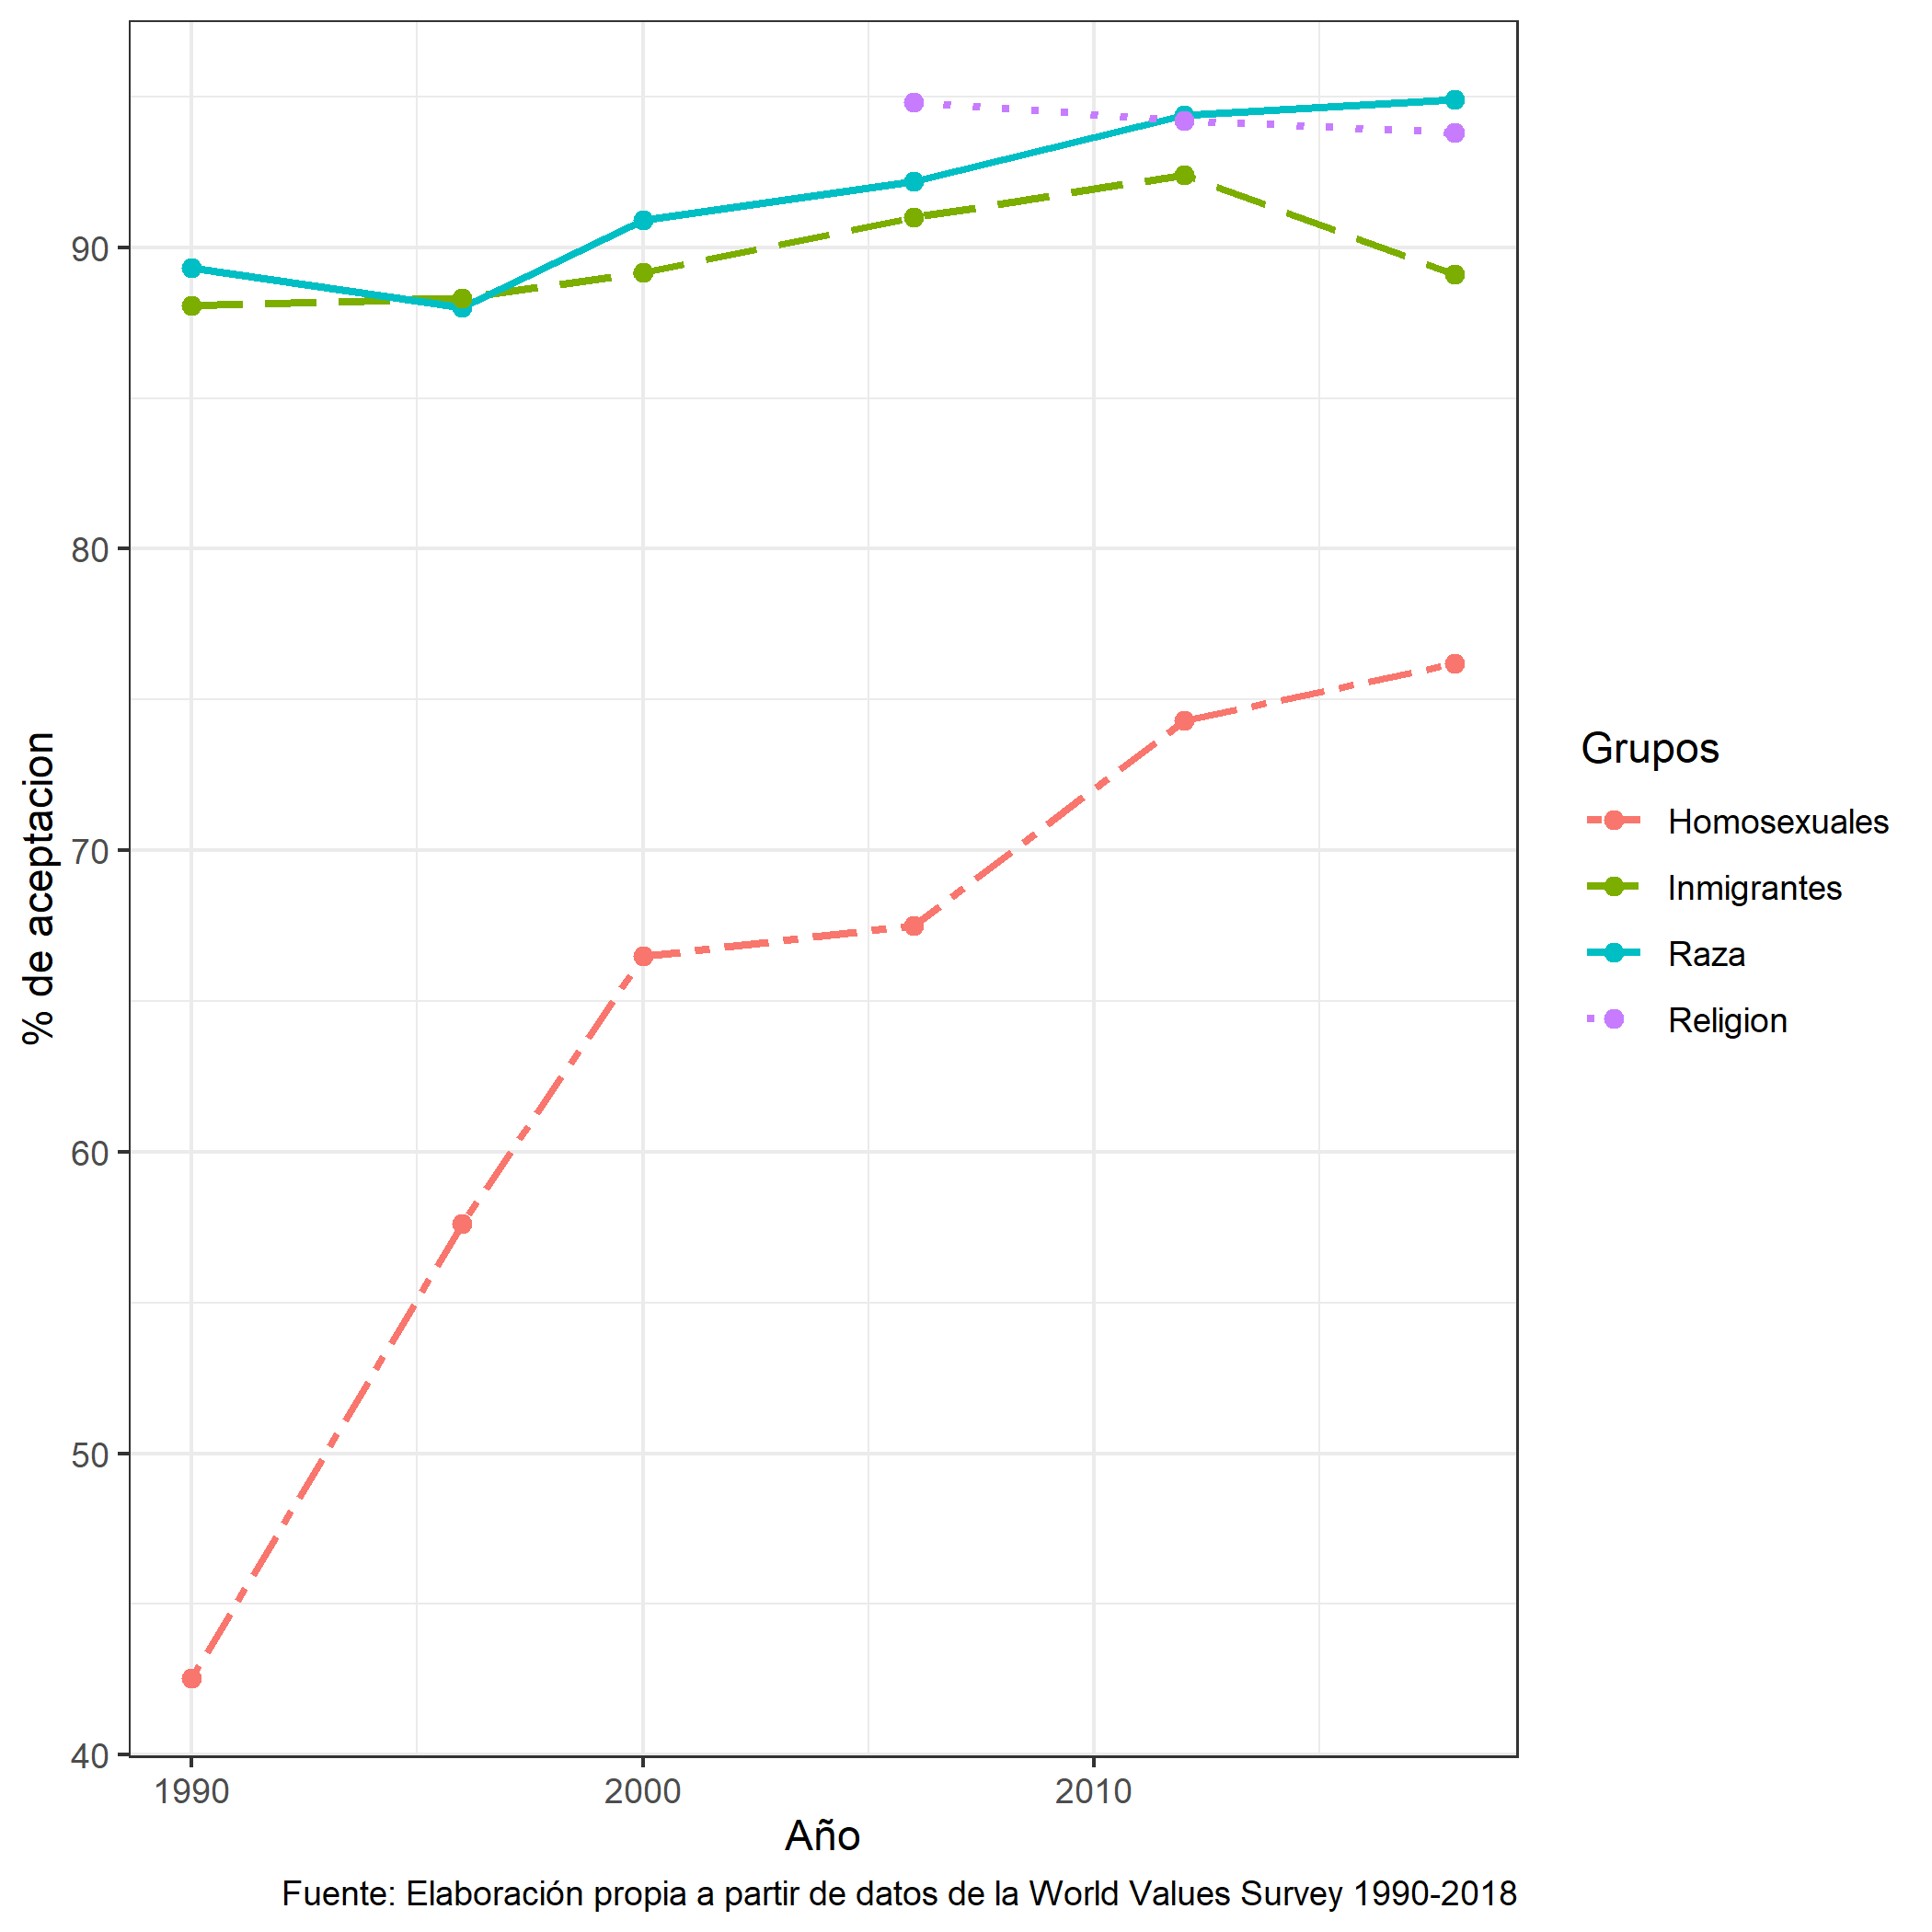
\includegraphics[width=1\linewidth]{images/aceptacion_wvs} 

}

\caption{Porcentaje de aceptación de distintos grupos sociales en población adulta de Chile}\label{fig:aceptacion-wvs}
\end{figure}

\textbf{Políticas educativas y los desafíos para la democracia actual}

Abordar el aprendizaje de actitudes hacia la aceptación social de jóvenes en edad escolar implica posicionar esta investigación bajo un incremento de la diversidad social que plantea importantes desafíos para los Estados-nación a nivel global en términos de políticas públicas, ya sea por sus implicancias gubernamentales, territoriales y socioeconómicas o por los nuevos requisitos que se originan en los distintos sistemas educativos a partir de demandas por inclusión y tolerancia de una población estudiantil diversa. En Chile se han suscrito distintos tratados internacionales que pretenden resguardar la diversidad (convenciones de DDHH, convenciones de Derechos del niño y el convenio 169 de la Organización Internacional del Trabajo) y que se han traducido en distintas políticas educativas que tienen por objetivo apoyar la inclusión de distintos sectores de la sociedad en el sistema educativo.

Dentro de este ámbito destacan la ley de inclusión escolar que regula, entre otras cosas, la admisión de los y las estudiantes en los establecimientos educativos \citep{bibliotecadelcongresonacional_ley_2015} y el Programa de Educación Intercultural Bilingüe (PEIB) que tiene sus orígenes en la década de 1990 y una consolidación entre 2010 y 2016 y que pretende generar las condiciones para que las comunidades educativas, que atienden a estudiantes indígenas y no indígenas, sean partícipes de procesos sociales inclusivos, que desarrollen nuevas competencias al considerar en sus procesos formativos otras formas de ver y entender el mundo y que reconozcan, valoren y se ajusten a estos orígenes culturales diversos \citep{ministeriodeeducacion_Programa_2017}.

Sumado a lo anterior, los aprendizajes que se le adjudican a la educación ciudadana en las escuelas pretenden dar respuesta a la necesidad de preparar a la nueva generación para la vida en democracia y sus requerimientos morales y cognitivos \citep{cox_objetivos_2015}. En este sentido, la nueva ley de Formación Ciudadana (ley n° 20.911) dispone que todos los establecimientos educacionales deben diseñar un Plan de Formación Ciudadana que brinde a los estudiantes la preparación necesaria para asumir una vida responsable en una sociedad libre y de orientación hacia el mejoramiento integral de la persona humana, como fundamento del sistema democrático, la justicia social y el progreso \citep{bibliotecadelcongresonacional_plan_2016}. Entre sus principales objetivos, esta nueva ley busca promover la comprensión y análisis del concepto de ciudadanía y los derechos y deberes asociados a ella, además de fomentar en los estudiantes la valoración de la diversidad social y cultural del país y fomentar en los estudiantes la tolerancia y el pluralismo \citep{bibliotecadelcongresonacional_plan_2016}.

Sin embargo, la tolerancia orientada hacia la existencia de una diversidad social marca una diferencia entre la aceptación, respeto y apreciación de la diferencia y la inclusión homogeneizante de los distintos grupos sociales dentro de las escuelas, ya que la definición de interculturalidad que se ha incluido en el sistema educativo es funcional al estatus quo al absorber a la diferencia y homogenizarlos \citep{riedemann_Desde_2020}. De esta forma, se invisibiliza y reproduce una discriminación basada en procesos de racialización, generización y diferenciación en términos de clase, acercándose más a la idea de multiculturalismo que a la de interculturalidad \citep{stefoni_Educacion_2016a}. Esta confusión en el horizonte de la educación intercultural produce una ineficacia de las políticas emprendidas y repercute en una incapacidad de generar una sociedad que acepte la diversidad y que establezca relaciones de cooperación entre sus diversidades \citep{donosoromo_INTERCULTURALIDAD_2006}. Lo anterior provoca que, en la práctica, antes que buscar una coexistencia de las diversidades, en el sistema educativo chileno se busca que los diferentes grupos sociales se integren a la sociedad nacional para que así obtengan los beneficios que ella reporta a todos sus ciudadanos \citep{donosoromo_INTERCULTURALIDAD_2006}. Esto, a su vez, provoca una contradicción en los establecimientos educacionales ya que se les pide valorar la diversidad social y cultural en las aulas mientras que, al mismo tiempo, se les exige responder a mecanismos de rendición de cuentas estandarizados que no dan cuenta de la diversidad \citep{riedemann_Desde_2020}.

De esta forma, si bien los procesos de socialización se han amplificado y complejizado junto con los procesos de modernización y globalización, el rol de la escuela y la familia siguen siendo los principales agentes de socialización. En este sentido, para la sociología la comprensión de la educación como un agente de socialización de las generaciones más jóvenes resulta fundamental, mientras que el rol de la familia ha sido estudiado en menor medida dentro de esta disciplina, sino más bien desde la psicología social. Así, las investigaciones sobre tolerancia e inclusión en población juvenil frecuentemente se han enfocado en problemáticas relacionadas con los flujos migratorios y su inserción en el sistema educativo de cada país, centrándose en cómo las escuelas permiten el ingreso e inclusión de distintos estudiantes en el sistema educativo \citep{bellei_estudio_2013, ortiz_Actitudes_2016, stefoni_Educacion_2016a} o en cómo las escuelas son capaces de influir en la (in)tolerancia y prejuicio hacia inmigrantes, minorías étnicas o disidencias sexuales \citep{lee_Tolerated_2014, maurissen_Classroom_2020, trevino_Influence_2018}. En la misma línea, en cuanto al rol de la familia, algunas investigaciones han dado cuenta del efecto de las actitudes de los padres en el conflicto interétnico de su descendencia \citep{medjedovic_intergroup_2021} y de la participación política parental en el compromiso político de las nuevas generaciones \citep{bacovsky_raising_2021}. Además, en sociedades desiguales como la chilena, los recursos socioeconómicos funcionan como un mecanismo de diferenciación a nivel general donde, por ejemplo, \citet{bellei_estudio_2013} ha dado cuenta del rol predominante de los recursos socioeconómicos de las familias como un agente diferenciador del logro académico.

Por lo tanto, resulta relevante comprender cómo los diferentes modos de socialización se articulan entre sí y producen las disposiciones para excluir o aceptar a determinados grupos sociales. Así, la pregunta de investigación que guía este estudio es ¿en qué medida los distintos procesos de socialización son capaces de influir en las actitudes de las y los jóvenes estudiantes chilenos hacia la diversidad en su vecindario?

\hypertarget{objetivo-general}{%
\section{Objetivo general}\label{objetivo-general}}

Determinar en qué medida varían las actitudes de los/as estudiantes que se relacionan con la aceptación de distintos grupos sociales de sus vecindarios, así como analizar el rol que poseen la familia y la escuela como agentes de socialización política de actitudes en jóvenes estudiantes chilenos.

\hypertarget{objetivos-especuxedficos}{%
\section{Objetivos específicos}\label{objetivos-especuxedficos}}

\begin{enumerate}
\def\labelenumi{\arabic{enumi}.}
\item
  Determinar en qué medida los/as jóvenes estudiantes chilenos aceptan o rechazan que diferentes grupos sociales vivan en sus vecindarios.
\item
  Analizar el rol de la familia en la socialización política de actitudes hacia la diversidad social.
\item
  Analizar el rol de la escuela en la socialización política de actitudes hacia la diversidad social.
\end{enumerate}

\hypertarget{antecedentes-teuxf3ricos-y-empuxedricos.}{%
\chapter{Antecedentes teóricos y empíricos.}\label{antecedentes-teuxf3ricos-y-empuxedricos.}}

\hypertarget{aceptar-la-diversidad-en-el-vecindario}{%
\section{Aceptar la diversidad en el vecindario}\label{aceptar-la-diversidad-en-el-vecindario}}

En Chile, las desigualdades interaccionales se han convertido en las desigualdades más percibidas y rechazadas por la población \citep{araujo_igualdad_2013}. Este tipo de desigualdades refieren a la manera en que las personas son tratadas por otros individuos o instituciones en las interacciones sociales ordinarias y concretas \citep{araujo_percepcion_2019}. En este sentido, para \citet{araujo_percepcion_2019} se ha instalado una \emph{malignización de la otredad}, en que se constituye al otro como una amenaza y adversario, quebrando la noción de un espacio común y dando un marco de confrontación y disputa a las relaciones ordinarias entre los habitantes de la ciudad. De esta forma, resulta relevante resaltar que, según \citet{castells_globalizacion_2005}, el principio identitario dominante en América Latina es la identidad nacional, construida en torno a un Estado-nación que impulsaba un proyecto de desarrollo y una especificidad frente al resto de los países. Así, en la medida en que el Estado-nación se inserta en la globalización y se despega de sus bases tradicionales, ``la separación entre Estado y nación lleva a una crisis de la identidad nacional como principio de cohesión social'' \citep[p.~40]{castells_globalizacion_2005}.

Como resultado, \citet{castells_globalizacion_2005} plantea que la identidad se convierte en un principio débil que no basta para construir el sentido de la vida colectiva y son suplantadas por el individualismo legitimado por el mercado, que se convierte en fuente de racionalidad y de proyecto, a la vez que se crean identidades comunitarias más fuertes, lo que conlleva el resurgimiento de la religión o identidades étnicas. Ante esta problemática, la Teoría de la Identidad Social ofrece un marco conceptual que permite explicar los procesos grupales y las relaciones intergrupales en términos de la interacción de los procesos sociales cognitivos, sociales interactivos y societarios, en el que se ubica la autoconcepción identitaria en el centro de esta dinámica \citep{hogg_social_2016}. Esta interacción intergrupal se concibe como un recurso funcional que emerge en el seno de condicionantes contextuales e individuales concretos con el objeto de proporcionar a cada individuo las estrategias necesarias para afirmar su identidad \citep{scandroglio_teoria_2008}. Así, esta construcción de una identidad social define y evalúa el autoconcepto de uno mismo y cómo será tratado y pensado por los demás y, por lo tanto, cuando las personas hacen comparaciones entre su propio grupo y un grupo externo, se preocupan por asegurarse de que su propio grupo sea positivamente distintivo, claramente diferenciado y evaluado más favorablemente que los grupos externos relevantes \citep{hogg_social_2016}.

De esta forma, la exclusión o rechazo de diferentes grupos sociales de un vecindario se comprende como una forma de cierre social en que se establecen barreras entre sectores o clases a partir de la construcción de identidades, comunidades y la monopolización de oportunidades con el fin de excluir a otras personas de ese círculo o clase \citep{parkin_Marxismo_1984}. En esta misma línea, \citet{tilly_desigualdad_2000} plantea que en cada sociedad existen desigualdades persistentes, ya que las desigualdades por ``raza, género, etnia, clase, edad, ciudadanía, nivel educacional y otros principios de diferenciación aparentemente contradictorios, se forman mediante procesos sociales similares y son, en una medida importante, organizacionalmente intercambiables'' \citep[p.~23]{tilly_desigualdad_2000}. Por un lado, estas desigualdades, más allá de las frecuentes formas de violencia explícitamente racista, tienden a materializarse en no tener acceso o tener un acceso menor al país, ciudad, barrio, vivienda, bares, política y/o medios de comunicación \citep{vandijk_Racismo_2013}. \citet{vandijk_Racismo_2013} señala que se trata de una práctica social diferenciada, generalmente denominada discriminación, que se basa en prejuicios e ideologías racistas sobre la superioridad de una mayoría y la inferioridad de una minoría. Por otro lado, \citet{diez-nicolas_Exclusion_2019} plantean que se trata de formas de exclusión social que frecuentemente se relacionan con conceptos como estigma, discriminación y prejuicio. No obstante, reducir o intensificar ciertas actitudes tendrá poco efecto sobre estas desigualdades persistentes, por lo que el foco debe estar puesto en los mecanismos sociales que producen esta desigualdad \citep{tilly_desigualdad_2000}

Sin embargo, medir la (in)tolerancia es un debate sostenido dentro de distintas disciplinas, que generalmente confluyen en dos enfoques centrales. Por un lado, se ha propuesto medir la tolerancia hacia grupos subalternos tales como migrantes, minorías étnicas y mujeres a partir de un enfoque de derechos \citep{miranda_Political_2018, trevino_Influence_2018}, de prejuicios \citep{meeusen_ParentChild_2015, weber_educational_2020} y como una amenaza material y/o simbólica \citep{raijman_Perceived_2004}. Por otro lado, \citet{diez-nicolas_Exclusion_2019} plantean que se trata de formas de exclusión social que frecuentemente se relacionan con conceptos como estigma, discriminación y prejuicio. Asimismo, \citet{tendam_Measuring_2011} proponen que, para jóvenes, las actitudes de ciudadanía se manifiestan en las tareas sociales cotidianas. En la presente investigación se propone medir la tolerancia a partir de la aceptación o rechazo de que distintos grupos sociales vivan en el mismo vecindario que los estudiantes encuestados. Aceptar la diversidad en el vecindario refiere, por lo tanto, a formas de no exclusión de distintos grupos subalternos tradicionalmente marginados de la esfera social. En concreto, esta perspectiva teórica permite abordar si los estudiantes aceptan o rechazan que vivan en su vecindario personas de origen indígena, de distinto país, distinta región, distinta orientación sexual, distinta clase social, distinto color de piel, distinta religión y con discapacidades físicas o mentales.

\hypertarget{procesos-de-socializaciuxf3n-poluxedtica-de-actitudes}{%
\section{Procesos de socialización política de actitudes}\label{procesos-de-socializaciuxf3n-poluxedtica-de-actitudes}}

A través de procesos de socialización diferenciados y continuos en el tiempo, es que se producen distintos condicionamientos asociados a una clase particular de condiciones de existencia \citep{bourdieu_sentido_2007}. A partir de esto, si bien los planteamientos de \citet{bourdieu_sentido_2007} podrían explicar la disposición de los individuos a generar y reproducir prácticas de exclusión social hacia distintos grupos sociales, no permiten comprender el modo en que se generan estas disposiciones. Es así como \citet{archer_teoria_2009} plantea la problemática que ha tenido la sociología de la educación al centrarse solo en las prácticas y procesos que ocurren dentro de la escuela y no reconocer que ``tanto los profesores como los alumnos están inmersos en relaciones socioculturales más amplias que traen consigo a la sala de clase'' \citep[p.~39]{archer_teoria_2009}. Esto implica que existe una interacción entre el contexto y las actividades sociales, pero que estas no covarían en el tiempo, sino que están desfasadas la una de la otra. En esta línea, para \citet{lahire_teoria_2012} resulta relevante comprender el mundo social a escala del individuo, al mismo tiempo que se comprenden las condiciones sociales (y discursivas) de producción del individuo moral e ideológico, porque son elementos socialmente producidos. En este caso, resulta relevante resaltar el objetivo de esta investigación en el sentido de comprender cómo los diferentes modos de socialización se articulan entre sí y producen las disposiciones para excluir o aceptar a determinados grupos sociales, ya que ``los individuos socializados pueden haber interiorizado de manera duradera un cierto número de hábitos y, sin embargo, no tener ningún deseo particular de aplicarlos'' \citep[p.~87]{lahire_teoria_2012}.

De esta forma, la sociología en general y la sociología de la educación en particular se concebirían como una sociología de los modos de socialización (escolares y extraescolares), articulándose con una sociología del conocimiento, para así poder comprender a grandes rasgos una disposición a partir de la reconstrucción de su génesis \citep{lahire_teoria_2012}. Esto es, abordar de manera articulada el rol de la familia y la escuela en la socialización política de actitudes hacia la diversidad social y el contexto en que estas se producen.

Al articular los diferentes modos de socialización, \citet{aedohenriquez_habitus_2015} señala que es relevante tener en consideración la idea de Estrategia de Bourdieu, ya que esta implica ponerse a sí mismo en relación con otros, en situaciones propias del campo, en que las expectativas socializadas sobre su posición con respecto a otros entran en interrogación. Asimismo, la idea de Estrategia de Bourdieu refiere a que ``en el mundo social actuamos conforme a ciertas inclinaciones que hemos incorporado a lo largo de nuestra experiencia social, en el marco de los procesos de socialización, inclinaciones o disposiciones que actúan como facilitadores de nuestras prácticas o de nuestros actos'' \citep[p.~280]{aguilar_habitus_2017}.

Así, los grupos familiares estratégicamente seleccionan escuelas y vecindarios en los que integrar a sus hijos de acuerdo con sus disposiciones, esto es, que son capaces de elegir el espacio social en que socializarán a sus hijos. De la misma forma, la disposición hacia la exclusión -y hacia el cierre social que conlleva- marcaría dos momentos temporales. Por un lado, refiere a una expresión de los procesos de socialización familiares previos y, por otro lado, expresan las condiciones familiares objetivas que condicionan el proceso de socialización actual.

\hypertarget{socializaciuxf3n-poluxedtica-familiar-de-actitudes-hacia-la-diversidad-social.}{%
\subsection{Socialización política familiar de actitudes hacia la diversidad social.}\label{socializaciuxf3n-poluxedtica-familiar-de-actitudes-hacia-la-diversidad-social.}}

El proceso de socialización política familiar se concibe como prácticas de crianza o estrategias de socialización concretas que buscan modelar las conductas de sus hijos e hijas, según las propias valoraciones y personalidades que se estimen como positivas para la integración y el desenvolvimiento social en el futuro \citep{ramirez_padres_2005}. De esta forma, las familias reproducen y socializan valores a través de un proceso de transmisión de actitudes que permite asegurar la perpetuación del grupo social y la conservación del estatus y el privilegio \citep{bourdieu_reproduccion_1998, bernstein_theoretical_2005}.

Dentro de las estrategias del proceso de socialización política familiar se han reconocido dos elementos fundamentales. En primer lugar, \citet{lipset_hombre_1997} plantea la importancia de las condiciones socioeconómicas objetivas de la familia en el proceso de adquisición de valores y prácticas democráticas. En segundo lugar, para \citet{bandura_sociallearning_1969} la teoría del aprendizaje social implica que las actitudes y comportamientos de los padres inciden sobre los intereses y modos de comportamiento de sus hijos, planteando así la importancia de la transmisión intergeneracional de actitudes como proceso de socialización.

En este sentido, diferentes investigaciones han dado cuenta del rol predominante que poseen los recursos socioeconómicos como condicionante de las expectativas de participación política de los estudiantes \citep{castillo_Social_2014} y, específicamente, sobre las actitudes de los estudiantes hacia uno o más grupos subalternos según el grado de tolerancia \citep{farkac_Tolerance_2020}, de prejuicios \citep{weber_educational_2020} o hacia la igualdad de derechos \citep{isac_Native_2012, miranda_Political_2018}. Por un lado, \citet{miranda_Political_2018} demuestran la importancia que posee el nivel educativo de los padres, el estatus ocupacional y la cantidad de libros en el hogar en la generación de actitudes positivas de los estudiantes hacia la igualdad de género y el estatus ocupacional de los padres y la cantidad de libros en el hogar sobre las actitudes hacia la igualdad de derechos para inmigrantes y minorías étnicas. Asimismo, \citet{ortiz_Actitudes_2016} demuestra la importancia que poseen estos tres indicadores sobre las actitudes hacia la tolerancia social en general, mientras que \citet{castillo_Social_2014} demuestran que padres con educación universitaria y la cantidad de libros en el hogar juegan un rol preponderante en las expectativas de participación política de los estudiantes. Por otro lado, \citet{sincer_relationship_2020} demuestran que una mayor proporción de estudiantes de bajo nivel socioeconómico en las escuelas influyen negativamente en las competencias para lidiar con las diferencias sociales\footnote{\citet{sincer_relationship_2020} señalan que \emph{dealing with differences} refiere al conocimiento, actitudes y habilidades para interactuar con las diferencias sociales.}. Por último, sobre la transmisión intergeneracional de actitudes, se ha dado cuenta de la preponderancia de las actitudes de los padres en la disposición hacia el conflicto interétnico de sus hijos \citep{medjedovic_intergroup_2021}, de cómo el historial de participación política parental influye en el compromiso político de las nuevas generaciones \citep{bacovsky_raising_2021} y que las familias de clase alta tienden a privilegiar valores más simbólico-relacionales, como los buenos modales y el respeto por los demás, mientras que las clases bajas privilegiarían transmitir valores de ascenso social, como el trabajo duro y el ahorro \citep{santanderramirez_preferencias_2020}. De esta forma, el proceso de socialización política familiar se refleja en las siguientes hipótesis:

\begin{itemize}
\item
  H1: Estudiantes que provienen de familias con mayores recursos socioeconómicos poseen un mayor grado de aceptación de la diversidad en sus vecindarios, manteniendo el resto de las variables constantes.
\item
  H2: Estudiantes que provengan de familias en que sus padres acepten en mayor medida que distintos grupos sociales vivan en sus vecindarios, poseerán un mayor grado de aceptación de la diversidad en sus vecindarios, manteniendo el resto de las variables constantes.
\end{itemize}

\hypertarget{socializaciuxf3n-poluxedtica-de-actitudes-hacia-la-diversidad-social-en-la-escuela.}{%
\subsection{Socialización política de actitudes hacia la diversidad social en la escuela.}\label{socializaciuxf3n-poluxedtica-de-actitudes-hacia-la-diversidad-social-en-la-escuela.}}

Dentro de la investigación sobre socialización política de actitudes en la escuela se tiende a adjudicar al sistema educacional el objetivo de ``suscitar y desarrollar al niño cierto número de estados físicos, intelectuales y morales que requieren en él tanto la sociedad política en su conjunto como el medio ambiente específico al que está especialmente destinado'' \citep[p.~60]{durkheim_educacion_1999}, y que la función socializadora de la escuela se resume en que ``consiste en el desarrollo dentro de cada individuo de aquellas habilidades y actitudes que constituyen los requisitos esenciales para su futuro desenvolvimiento en la vida'' \citep[p.~65]{parsons_clase_1976}. En esta línea, investigaciones recientes continúan enmarcándose en este rol de la escuela como agente formador de ciudadanos \citep{cox_Aprendizaje_2015, groof_Influence_2008, trevino_Influence_2017}, resaltando las capacidades que tienen las escuelas para contribuir en el desarrollo cívico y las actitudes democráticas de los jóvenes estudiantes.

De esta forma la escuela se comprende como el espacio primordial de socialización y de encuentro entre personas de distintas realidades, funcionando como una micro sociedad \citep{groof_Influence_2008}. Así, las características estructurales de las escuelas son una dimensión clave para explicar los diferentes resultados que poseen los estudiantes \citep{trevino_Influence_2018}. En cierta medida esto se explica por la forma en que los estudiantes de diferentes estratos socioeconómicos se distribuyen a través de las escuelas según su tipo de administración \citep{bellei_estudio_2013} y por los conocimientos, habilidades y valores sociales que estas instituciones le logran otorgar a sus estudiantes \citep{groof_Influence_2008}. Específicamente, tanto las escuelas como las salas de clases pueden diferir entre sí en cuanto a sus valores y normas comunes, en cómo los estudiantes interactúan entre sí y cómo los profesores se acercan y tratan a los estudiantes \citep{bayramozdemir_How_2020}.

En primer lugar, el conocimiento cívico y las oportunidades que brinden las escuelas para su aprendizaje es un elemento esencial para la socialización de valores y normas comunes. El conocimiento cívico refiere a la información cívica y ciudadana aprendida que los estudiantes utilizan cuando se involucran en tareas más complejas que les ayudan a entender de mejor forma el mundo político \citep{carstens_Overview_2018}. Diversos autores han demostrado que el conocimiento cívico influye de manera positiva sobre las actitudes de estudiantes hacia la tolerancia de personas inmigrantes \citep{isac_Native_2012, groof_Influence_2008, torney-purta_How_2008}, mientras que \citet{sampermans_Back_2020} señalan que el conocimiento cívico depende directamente de las oportunidades de aprendizaje cívico que logren promover las escuelas.

En segundo lugar, una de las características estructurales fundamentales de las escuelas es la disposición de espacios de discusión. En las aulas donde los estudiantes están expuestos al mundo real de los problemas políticos, por medio del discurso y el debate tienen la oportunidad de luchar por cuestiones políticas y sociales, aprendiendo el elemento vital de la democracia participativa \citep{campbell_Voice_2008}. Por lo tanto, es evidente que esto solo se puede lograr cuando se promueve y se resguarda que exista comunicación y diálogo entre los alumnos de diferentes nacionalidades, etnias, lenguas, colores de piel, estratos socioeconómicos e intereses \citep{riedemann_Desde_2020}. Se ha demostrado que este indicador influye sobre las actitudes de los estudiantes hacia la tolerancia de inmigrantes \citep{maurissen_Classroom_2020, groof_Influence_2008, isac_Native_2012}, sobre las actitudes de los estudiantes hacia la igualdad de derechos para inmigrantes, minorías étnicas y mujeres \citep{trevino_Influence_2018, trevino_Influence_2017}, sobre las actitudes cívicas de los estudiantes en general \citep{barber_Profiles_2020} y sobre la formación de conocimiento cívico en los estudiantes \citep{sampermans_Back_2020, barber_Immigrant_2015}. De esta forma, el rol de la escuela en la socialización política de actitudes se resume en las siguientes hipótesis:

\begin{itemize}
\item
  H3: Estudiantes que poseen un mayor conocimiento cívico presentan un mayor grado de aceptación de la diversidad en sus vecindarios, manteniendo el resto de las variables constantes.
\item
  H4: Estudiantes que perciben una mayor apertura a la discusión en sus aulas presentan un mayor grado de aceptación de la diversidad en sus vecindarios, manteniendo el resto de las variables constantes.
\end{itemize}

Finalmente, debido al rol del sistema educacional al alero de las nuevas políticas públicas de inclusión y Educación ciudadana, de manera exploratoria se plantea que las escuelas son capaces de mitigar las desigualdades sociales de origen o potenciar las actitudes positivas en la formación de las actitudes de los estudiantes hacia la aceptación de la diversidad en sus vecindarios. Esto implica que las escuelas cumplen un rol moderador en la generación de las actitudes de los estudiantes y, por lo tanto, se plantea la siguiente hipótesis:

\begin{itemize}
\tightlist
\item
  H5: El proceso de socialización en las escuelas cumple un rol moderador sobre la influencia de la socialización de la familia en las actitudes de los estudiantes hacia la aceptación de la diversidad en sus vecindarios.
\end{itemize}

\hypertarget{implicancias-del-vecindario-en-la-socializaciuxf3n-poluxedtica-de-actitudes-hacia-la-diversidad-social.}{%
\subsection{Implicancias del vecindario en la socialización política de actitudes hacia la diversidad social.}\label{implicancias-del-vecindario-en-la-socializaciuxf3n-poluxedtica-de-actitudes-hacia-la-diversidad-social.}}

El incremento de la diversidad social en los vecindarios tiene distintos efectos sobre la convivencia social y la tolerancia de lo que se percibe como diferente. Por un lado, en vecindarios heterogéneos, con una mayor diversidad de contactos sociales y una mayor interacción entre individuos de diversos orígenes, se deberían generar las condiciones para tener un mayor grado de prosocialidad \citep{diprete_segregation_2011}, sin embargo, también se ha argumentado que una mayor interacción entre grupos distintos podría reforzar los prejuicios \citep{putnam_pluribus_2007}. Por otro lado, la marcada segregación urbana del contexto chileno que sienta las bases para la consolidación de vecindarios homogéneos es bastante desfavorable para el contacto intergrupal positivo y la reducción de prejuicios \citep{garreton_city_2017}. En esta misma línea, \citet{garreton_social_2021} muestran que el capital social, es decir, una mayor cantidad de vínculos y contactos positivos, está negativamente correlacionado con la diversidad socioeconómica, pero positivamente correlacionado con una mayor diversidad de inmigrantes, lo que sugiere la importancia de diferenciar ambos contextos en el desarrollo del capital social.

En cada vecindario, los distintos patrones de segregación están asociados con grandes diferencias en el acceso al mercado laboral y a otros recursos culturales y sociales \citep{fernandez_breaking_2016}. Así, según \citet{baldassarri_diversity_2020}, la competencia entre \emph{minorías} es mayor en los lugares donde estas son más numerosas. Esto se debe a que las minorías étnicas y raciales a menudo no pueden competir por trabajos de alta calidad, incluso estando calificadas para ellos, y en su lugar se ven obligadas a competir por trabajos de menor calidad o informales, lo que trae como consecuencia que las personas de clases sociales bajas puedan sentir a las minorías como amenazas con más frecuencia que la gente de clases sociales más altas \citep{baldassarri_diversity_2020}. Este sentimiento de amenaza producido por la competencia por recursos y trabajos tiende a disminuir la confianza entre grupos distintos, dificultando así el desarrollo de vínculos sociales \citep{cote_untangling_2009}.

De esta forma, las características específicas de cada vecindario podrían afectar de diferentes maneras las actitudes de los y las estudiantes, dependiendo de sus condiciones materiales, de la disponibilidad de recursos y de la calidad y cantidad de los contactos e interacciones con personas de diferentes grupos. Sin embargo, algunos de estos elementos escapan de los alcances de esta investigación y de la disponibilidad de datos, por lo que se plantean tres hipótesis sobre características de los vecindarios que podrían afectar si los y las estudiantes aceptan o rechazan que distintos grupos sociales vivan en sus vecindarios:

\begin{itemize}
\item
  H6: Estudiantes que viven en vecindarios con un mayor índice de diversidad étnica presentan un menor grado de aceptación de la diversidad en sus vecindarios, manteniendo el resto de las variables constantes.
\item
  H7: Estudiantes que viven en vecindarios con un mayor índice de población inmigrante presentan un menor grado de aceptación de la diversidad en sus vecindarios, manteniendo el resto de las variables constantes.
\item
  H8: Estudiantes que viven en vecindarios con un mayor promedio de escolaridad mayor presentan un mayor grado de aceptación de la diversidad en sus vecindarios, manteniendo el resto de las variables constantes.
\end{itemize}

\hypertarget{metodologuxeda}{%
\chapter{Metodología}\label{metodologuxeda}}

\hypertarget{datos}{%
\section{Datos}\label{datos}}

La base de datos a utilizar corresponde al Primer Estudio de Educación Ciudadana en Chile, realizado por la Agencia de Calidad de la Educación del Ministerio de Educación. En este estudio se evaluaron 8.701 estudiantes de octavo básico provenientes de 242 escuelas. La fecha de aplicación fue el 9 de noviembre de 2017.

En la base de datos disponible, se cuenta con 10.213 estudiantes que poseen puntajes en la prueba de conocimiento cívico (9 variables). De este total, el cuestionario completo de estudiantes posee 8.589 respuestas (222 variables) y, de estos estudiantes, se poseen las respuestas de 6.770 apoderados (141 variables).

\hypertarget{variables}{%
\section{Variables}\label{variables}}

Con el fin de medir las actitudes de los y las estudiantes hacia la diversidad en sus vecindarios se utiliza la variable de ``Tolerancia y Distancia Social'' del cuestionario de estudiantes. Esta variable está medida a partir de las preguntas que se presentan en la Tabla \ref{tab:aceptacion-est}.

En relación con las variables independientes, para medir los recursos socioeconómicos de la familia se utilizará la cantidad de libros presentes en el hogar reportada por los estudiantes y el nivel educacional reportado por los apoderados. Además, se incluye la misma variable de ``Tolerancia y Distancia Social'' presente en el cuestionario de apoderados para analizar el efecto de la transmisión intergeneracional de actitudes. Asimismo, se utiliza la variable de puntaje de conocimiento cívico de los estudiantes y su percepción sobre la apertura a la discusión en el aula de clases.

\hypertarget{muxe9todos}{%
\section{Métodos}\label{muxe9todos}}

La metodología planteada para realizar esta investigación es de carácter cuantitativa. En primer lugar, debido a que las variables sobre la apertura a la discusión en el aula de clases son seis, se evaluará su dimensionalidad a partir de un Análisis Factorial Exploratorio (AFE), con el fin de determinar si se trata (o no) de una sola dimensión latente. Este análisis factorial exploratorio permite generar una sola escala que será utilizada como variable independiente.

En segundo lugar, se realizarán análisis descriptivos de todas las variables utilizadas en el estudio y análisis correlacionales para evaluar las asociaciones correspondientes a las hipótesis 1, 2, 3, 4 y 5. En tercer lugar, debido a que la muestra posee una estructura jerárquica de estudiantes anidados en escuelas, se estimarán regresiones multinivel para evaluar todas las hipótesis. Realizar una regresión multinivel permite aislar los efectos individuales (estudiantes) de los agregados (escuelas) y, a partir de esto, analizar la varianza de los resultados en cada nivel, así como la proporción de la varianza explicada por las variables independientes de cada nivel. Debido a que las características estructurales de las escuelas son una dimensión clave para explicar los diferentes resultados que poseen los estudiantes \citep{trevino_Influence_2018} y porque tanto las escuelas como las salas de clases pueden diferir entre sí en cuanto a sus valores y normas comunes \citep{bayramozdemir_How_2020}, se hace necesario estimar regresiones multinivel que permitan determinar si los resultados en las actitudes de los estudiantes dependen de sus respuestas a nivel individual o por características agregadas a nivel de escuela.

\hypertarget{anuxe1lisis}{%
\chapter{Análisis}\label{anuxe1lisis}}

\hypertarget{variables-independientes}{%
\section{Variables independientes}\label{variables-independientes}}

\textbf{Estudiantes}

\textbf{Apoderados}

\hypertarget{conclusiones}{%
\chapter{Conclusiones}\label{conclusiones}}

\hypertarget{bibliografuxeda}{%
\chapter*{Bibliografía}\label{bibliografuxeda}}
\addcontentsline{toc}{chapter}{Bibliografía}

% %%%%%%%%%%%%%%%%%%%%%%%%%%%%%%%%%%%%%%%%%%%%%%%%%
% %%% Bibliography                              %%%
% %%%%%%%%%%%%%%%%%%%%%%%%%%%%%%%%%%%%%%%%%%%%%%%%%
% \addtocontents{toc}{\vspace{.5\baselineskip}}
% \cleardoublepage
% \phantomsection
% \addcontentsline{toc}{chapter}{\protect\numberline{}{Bibliography}}
\bibliography{tesis}

%% All books from our library (SfS) are already in a BiBTeX file
%% (Assbib). You can use Assbib combined with your personal BiBTeX file:
%% \bibliography{Myreferences,Assbib}. Of course, this will only work on
%% the computers at SfS, unless you copy the Assbib file
%%  --> /u/sfs/bib/Assbib.bib



\end{document}
